\providecommand{\qcor}[1]{\ulcorner#1\urcorner}   %
\providecommand{\qcOne}{\mathbf{1}}   %
\providecommand{\evid}[1]{\mathrm{ev}_{\qcor{\mathrm{id}_{#1}}}}   %

\subsection*{练习}

\begin{exercise}\label{ex:pullback-cartesian-functors}
考虑一张图表，其中 $h$ 与 $k$ 分别在从 $A$ 到 $B$ 的诸\trTwoSidedFibration{}%
之间、以及从 $B$ 到 $C$ 的诸\trTwoSidedFibration{}之间定义\trCartesianFunctor{}：
\begin{center}
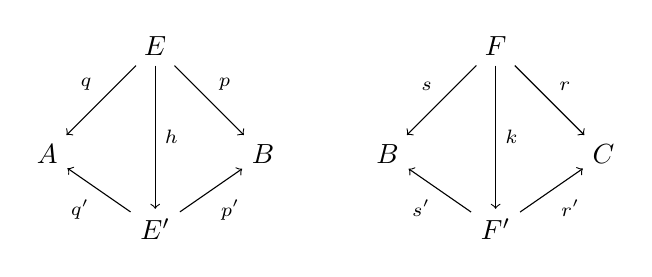
\begin{tikzpicture}[x=1.5em,y=1.5em]
  \begin{scope}[shift={(0,0)}]
    \node (E)  at (0,1.6) {$E$};
    \node (A)  at (-2.6,-1.0) {$A$};
    \node (B)  at (2.6,-1.0) {$B$};
    \node (Ep) at (0,-2.8) {$E'$};
    \draw[->] (E) -- node[above left]{$\scriptstyle q$} (A);
    \draw[->] (E) -- node[above right]{$\scriptstyle p$} (B);
    \draw[->] (E) -- node[right]{$\scriptstyle h$} (Ep);
    \draw[->] (Ep) -- node[below left]{$\scriptstyle q'$} (A);
    \draw[->] (Ep) -- node[below right]{$\scriptstyle p'$} (B);
  \end{scope}
  \begin{scope}[shift={(8.2,0)}]
    \node (F)  at (0,1.6) {$F$};
    \node (B2) at (-2.6,-1.0) {$B$};
    \node (C)  at (2.6,-1.0) {$C$};
    \node (Fp) at (0,-2.8) {$F'$};
    \draw[->] (F) -- node[above left]{$\scriptstyle s$} (B2);
    \draw[->] (F) -- node[above right]{$\scriptstyle r$} (C);
    \draw[->] (F) -- node[right]{$\scriptstyle k$} (Fp);
    \draw[->] (Fp) -- node[below left]{$\scriptstyle s'$} (B2);
    \draw[->] (Fp) -- node[below right]{$\scriptstyle r'$} (C);
  \end{scope}
\end{tikzpicture}
\end{center}
证明：$h$ 与 $k$ 经\trPullback{}可定义出一个介于从 $A$ 到 $C$ 的%
\trTwoSidedFibration{}之间的\trCartesianFunctor
$(h,k)\colon E\times_{B}F\to E'\times_{B}F'$。
\end{exercise}

\section{双侧 Yoneda 引理}\label{sec:two-sided-yoneda-lemma}

在本节中，我们将证明\trYonedaLemma{}的一个双侧版本，所借助的是可表示双侧纤维化%
的如下概念：

\begin{definition}\label{def:represented-two-sided-fibration}
对\trGeneralizedElement{}的任意一个跨度
$A\overset{a}{\leftarrow}X\overset{b}{\rightarrow}B$，如下跨度
\begin{center}
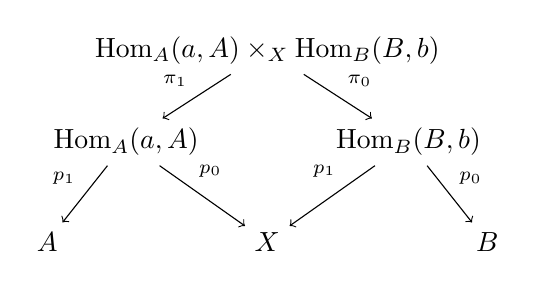
\begin{tikzpicture}[x=1.5em,y=1.5em]
  \node (P)  at (3.4,2.6) {$\mathrm{Hom}_{A}(a,A)\times_{X}\mathrm{Hom}_{B}(B,b)$};
  \node (HA) at (0,0.4) {$\mathrm{Hom}_{A}(a,A)$};
  \node (HB) at (6.8,0.4) {$\mathrm{Hom}_{B}(B,b)$};
  \node (A)  at (-1.9,-2.0) {$A$};
  \node (X)  at (3.4,-2.0) {$X$};
  \node (B)  at (8.7,-2.0) {$B$};
  \draw[->] (P) -- node[above left]{$\scriptstyle\pi_{1}$} (HA);
  \draw[->] (P) -- node[above right]{$\scriptstyle\pi_{0}$} (HB);
  \node at (3.4,1.5) {$\scriptstyle\llcorner$};
  \draw[->] (HA) -- node[above left]{$\scriptstyle p_{1}$} (A);
  \draw[->] (HA) -- node[above right,pos=0.35]{$\scriptstyle p_{0}$} (X);
  \draw[->] (HB) -- node[above left,pos=0.35]{$\scriptstyle p_{1}$} (X);
  \draw[->] (HB) -- node[above right]{$\scriptstyle p_{0}$} (B);
\end{tikzpicture}
\end{center}
定义了从 $A$ 到 $B$ 的一条\trTwoSidedFibration{}，我们称之为\textbf{由 $a$ 与 $b$
表示的双侧纤维化}（two-sided fibration represented by $a$ and $b$）。与单侧可%
表示物的情形一样，在 $(a,b)\colon X\to A\times B$ 之上的\trFiber{}中存在一个
典范的\trGeneralizedElement{}
$(\qcor{\mathrm{id}_{a}},\qcor{\mathrm{id}_{b}})\colon X\to\mathrm{Hom}_{A}(a,A)\times_{X}\mathrm{Hom}_{B}(B,b)$。
\end{definition}

\cref{def:represented-two-sided-fibration}的这一术语由双侧纤维化的那个%
\trYonedaLemma{}所证成，而后者我们将使用\cref{cor:generalized-yoneda-lemma}的
广义元素之\trYonedaLemma{}来证明。

\begin{theorem}[\trYonedaLemma]\label{thm:two-sided-yoneda-lemma}
对任意跨度 $A\overset{a}{\leftarrow}X\overset{b}{\rightarrow}B$ 与任意%
\trTwoSidedFibration{}
$A\overset{q}{\twoheadleftarrow}E\overset{p}{\twoheadrightarrow}B$，沿元素
$(\qcor{\mathrm{id}_{a}},\qcor{\mathrm{id}_{b}})\colon X\to\mathrm{Hom}_{A}(a,A)\times_{X}\mathrm{Hom}_{B}(B,b)$ 的限制定义了%
\trQuasiCategory{}之间的一个\trEquivalence
{\small\[
\mathrm{Fun}_{A\times B}^{\mathrm{cart}}\!\left(
\begin{gathered}
\mathrm{Hom}_{A}(a,A)\times_{X}\mathrm{Hom}_{B}(B,b)\\[-2pt]
\downarrow\scriptstyle (p_{1}\pi_{1},\,p_{0}\pi_{0})\\[-2pt]
A\times B
\end{gathered}
\;\right.,
\left.
\begin{gathered}
E\\[-2pt]
\downarrow\scriptstyle (q,\,p)\\[-2pt]
A\times B
\end{gathered}
\right)
\xrightarrow[\ \sim\ ]{\ \mathrm{ev}_{(\qcor{\mathrm{id}_{a}},\,\qcor{\mathrm{id}_{b}})}\ }
\mathrm{Fun}_{A\times B}\!\left(
\begin{gathered}
X\\[-2pt]
\downarrow\scriptstyle (a,\,b)\\[-2pt]
A\times B
\end{gathered}
\;\right.,
\left.
\begin{gathered}
E\\[-2pt]
\downarrow\scriptstyle (q,\,p)\\[-2pt]
A\times B
\end{gathered}
\right)
\]}
\end{theorem}

\begin{proof}
我们以定理 7.1.4(i) 的视角来证明这一结果：在∞-宇宙 $\mathcal{K}$ 中，把作为靶子
的\trTwoSidedFibration{}
$A\overset{q}{\twoheadleftarrow}E\overset{p}{\twoheadrightarrow}B$ 视为
∞-宇宙 $\mathrm{co}\mathcal{C}\mathit{art}(\mathcal{K})_{/A}$\footnote{原书印作 $\mathrm{co}\mathcal{C}\mathit{art}(\mathcal{K})_{/A\times B}$，按定理 7.1.4(i) 与下文自述应为 $\mathrm{co}\mathcal{C}\mathit{art}(\mathcal{K})_{/A}$，此处径改。——译者注}中
$\pi\colon A\times B\twoheadrightarrow A$ 之上的一条\trCartesianFibration{}。我们
通过两次施用\cref{cor:generalized-yoneda-lemma}来推导这一结果：先对
$\mathrm{co}\mathcal{C}\mathit{art}(\mathcal{K})_{/A}$ 中 $\pi\colon A\times B\twoheadrightarrow A$
之上的诸\trCartesianFibration{}施用，再对 $\mathcal{K}$ 中 $A$ 之上的诸%
\trCocartesianFibration{}施用。

为给 Yoneda 引理的第一次应用做准备，我们需要在 $\mathrm{co}\mathcal{C}\mathit{art}(\mathcal{K})_{/A}$
中，从 $A$ 之上的映射
\begin{rveq}\label{eq:span-over-a}
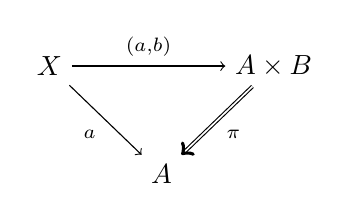
\begin{tikzpicture}[x=1.5em,y=1.5em]
  \node (X)  at (0,1.3) {$X$};
  \node (AB) at (5.4,1.3) {$A\times B$};
  \node (A)  at (2.7,-1.3) {$A$};
  \draw[->] (X) -- node[above]{$\scriptstyle(a,b)$} (AB);
  \draw[->] (X) -- node[below left]{$\scriptstyle a$} (A);
  \draw[double,->] (AB) -- node[below right]{$\scriptstyle\pi$} (A);
\end{tikzpicture}
\end{rveq}
出发，造出一个余定义域为 $\pi\colon A\times B\twoheadrightarrow A$ 的%
\trGeneralizedElement{}。\cref{cor:generalized-yoneda-lemma}给出一个\trEquivalence
\[
\mathrm{Fun}_{A}^{\mathrm{cart}}\bigl(
\mathrm{Hom}_{A}(a,A)\mathrel{\overset{p_{1}}{\twoheadrightarrow}}A,\,
A\times B\mathrel{\overset{\pi}{\twoheadrightarrow}}A
\bigr)
\xrightarrow[\ \sim\ ]{\ \mathrm{ev}_{\qcor{\mathrm{id}_{a}}}\ }
\mathrm{Fun}_{A}\bigl(
X\xrightarrow{\ a\ }A,\,
A\times B\mathrel{\overset{\pi}{\twoheadrightarrow}}A
\bigr)
\]
它告诉我们：$a\colon X\to A$ 在 $\mathrm{co}\mathcal{C}\mathit{art}(\mathcal{K})_{/A}$ 中的反射由
$p_{1}\colon\mathrm{Hom}_{A}(a,A)\twoheadrightarrow A$ 给出。于是我们取广义元素
为诸\trCocartesianFibration{}之间的如下\trCartesianFunctor
\begin{rveq}\label{eq:cartesian-functor-pair}
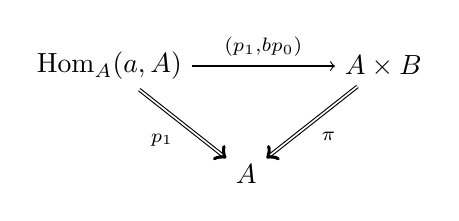
\begin{tikzpicture}[x=1.5em,y=1.5em]
  \node (H)  at (0,1.3) {$\mathrm{Hom}_{A}(a,A)$};
  \node (AB) at (6.6,1.3) {$A\times B$};
  \node (A)  at (3.3,-1.3) {$A$};
  \draw[->] (H) -- node[above]{$\scriptstyle(p_{1},bp_{0})$} (AB);
  \draw[double,->] (H) -- node[below left]{$\scriptstyle p_{1}$} (A);
  \draw[double,->] (AB) -- node[below right]{$\scriptstyle\pi$} (A);
\end{tikzpicture}
\end{rveq}
它沿 $\qcor{\mathrm{id}_{a}}\colon X\to\mathrm{Hom}_{A}(a,A)$ 的限制即
\eqref{eq:span-over-a}。

由\cref{cor:generalized-yoneda-lemma}再一次，对象 \eqref{eq:cartesian-functor-pair}
从 $(\mathrm{co}\mathcal{C}\mathit{art}(\mathcal{K})_{/A})_{/\pi\colon A\times B\twoheadrightarrow A}$
到 ${}_{A\backslash}\mathcal{F}\mathit{ib}(\mathcal{K})_{/B}$ 的反射，由其右逗号表示%
（该表示形成于 $\mathrm{co}\mathcal{C}\mathit{art}(\mathcal{K})_{/A}$ 中）的余定义域投影给出。这
复原出\trTwoSidedFibration
\begin{center}
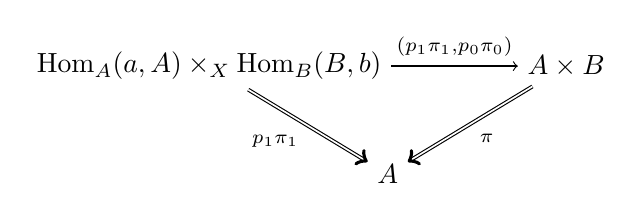
\begin{tikzpicture}[x=1.5em,y=1.5em]
  \node (P)  at (0,1.3) {$\mathrm{Hom}_{A}(a,A)\times_{X}\mathrm{Hom}_{B}(B,b)$};
  \node (AB) at (8.6,1.3) {$A\times B$};
  \node (A)  at (4.3,-1.3) {$A$};
  \draw[->] (P) -- node[above]{$\scriptstyle(p_{1}\pi_{1},p_{0}\pi_{0})$} (AB);
  \draw[double,->] (P) -- node[below left]{$\scriptstyle p_{1}\pi_{1}$} (A);
  \draw[double,->] (AB) -- node[below right]{$\scriptstyle\pi$} (A);
\end{tikzpicture}
\end{center}
于是，该结果给出一个\trEquivalence
{\small\[
\mathrm{Fun}_{A\times B}^{\mathrm{cart}}\!\left(
\begin{gathered}
\mathrm{Hom}_{A}(a,A)\times_{X}\\[-2pt]
\mathrm{Hom}_{B}(B,b)\\[-2pt]
\downarrow\scriptstyle (p_{1}\pi_{1},\,p_{0}\pi_{0})\\[-2pt]
A\times B
\end{gathered}
\;\right.,
\left.
\begin{gathered}
E\\[-2pt]
\downarrow\scriptstyle (q,\,p)\\[-2pt]
A\times B
\end{gathered}
\right)
\xrightarrow[\ \sim\ ]{\ \mathrm{ev}_{(\qcor{\mathrm{id}_{a}},\,\qcor{bp_{0}})}\ }
\mathrm{Fun}_{A\times B}^{\mathrm{cart}}\!\left(
\begin{gathered}
\mathrm{Hom}_{A}(a,A)\\[-2pt]
\downarrow\scriptstyle (p_{1},\,bp_{0})\\[-2pt]
A\times B
\end{gathered}
\;\right.,
\left.
\begin{gathered}
E\\[-2pt]
\downarrow\scriptstyle (q,\,p)\\[-2pt]
A\times B
\end{gathered}
\;\right)
\]}
其中右边的\trFunctorSpace{}由 $\mathrm{co}\mathcal{C}\mathit{art}(\mathcal{K})_{/A}$ 中%
\trFunctorSpace{}的如下\trPullback{}定义
\begin{center}
\begin{tikzpicture}[x=1.3em,y=1.3em,every node/.style={font=\small}]
  \node (NW) at (0,1.7) {$\mathrm{Fun}_{A\times B}^{\mathrm{cart}}\bigl(\mathrm{Hom}_{A}(a,A),\,E\bigr)$};
  \node (NE) at (10.4,1.7) {$\mathrm{Fun}_{A}^{\mathrm{cart}}\bigl(\mathrm{Hom}_{A}(a,A)\mathrel{\overset{p_{1}}{\twoheadrightarrow}}A,\,E\mathrel{\overset{q}{\twoheadrightarrow}}A\bigr)$};
  \node (SW) at (0,-1.7) {$\qcOne$};
  \node (SE) at (10.4,-1.7) {$\mathrm{Fun}_{A}^{\mathrm{cart}}\bigl(\mathrm{Hom}_{A}(a,A)\mathrel{\overset{p_{1}}{\twoheadrightarrow}}A,\,A\times B\mathrel{\overset{\pi}{\twoheadrightarrow}}A\bigr)$};
  \draw[->] (NW) -- (NE);
  \draw[->] (NW) -- (SW);
  \draw[->] (SW) -- node[above,pos=0.28]{$\scriptstyle(p_{1},bp_{0})$} (SE);
  \draw[->] (NE) -- node[right]{$\scriptstyle(q,p)_{*}$} (SE);
  \node at (0.5,0.9) {$\scriptstyle\llcorner$};
\end{tikzpicture}
\end{center}
\cref{cor:generalized-yoneda-lemma}又一次给出自然等价
\begin{center}
\begin{tikzpicture}[x=1.2em,y=1.3em,every node/.style={font=\small}]
  \node (TL) at (0,1.7) {$\mathrm{Fun}_{A}^{\mathrm{cart}}\bigl(\mathrm{Hom}_{A}(a,A)\mathrel{\overset{p_{1}}{\twoheadrightarrow}}A,\,E\mathrel{\overset{q}{\twoheadrightarrow}}A\bigr)$};
  \node (TR) at (10.6,1.7) {$\mathrm{Fun}_{A}\bigl(X\xrightarrow{\ a\ }A,\,E\mathrel{\overset{q}{\twoheadrightarrow}}A\bigr)$};
  \node (BL) at (0,-1.7) {$\mathrm{Fun}_{A}^{\mathrm{cart}}\bigl(\mathrm{Hom}_{A}(a,A)\mathrel{\overset{p_{1}}{\twoheadrightarrow}}A,\,A\times B\mathrel{\overset{\pi}{\twoheadrightarrow}}A\bigr)$};
  \node (BR) at (10.6,-1.7) {$\mathrm{Fun}_{A}\bigl(X\xrightarrow{\ a\ }A,\,A\times B\mathrel{\overset{\pi}{\twoheadrightarrow}}A\bigr)$};
  \draw[->] (TL) -- node[above]{$\scriptstyle\mathrm{ev}_{\qcor{\mathrm{id}_{a}}}$} node[below]{$\scriptstyle\sim$} (TR);
  \draw[->] (BL) -- node[above]{$\scriptstyle\mathrm{ev}_{\qcor{\mathrm{id}_{a}}}$} node[below]{$\scriptstyle\sim$} (BR);
  \draw[->] (TL) -- node[left]{$\scriptstyle(q,p)_{*}$} (BL);
  \draw[->] (TR) -- node[right]{$\scriptstyle(q,p)_{*}$} (BR);
\end{tikzpicture}
\end{center}
它们诱导出：左手边的\trIsofibration{}在 $(p_{1},bp_{0})$ 之上的\trFiber{}与
右手边的\trIsofibration{}在
$(p_{1},bp_{0})\cdot\qcor{\mathrm{id}_{a}}=(a,b)$ 之上的\trFiber{}之间的一个%
\trEquivalence{}。为计算这一\trFiber{}，请注意右手边的\trIsofibration{}本身就是
如下\trPullback
\begin{center}
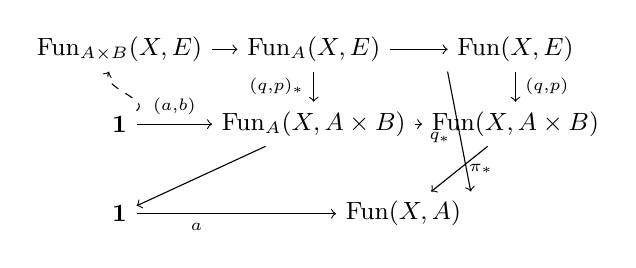
\begin{tikzpicture}[x=1.35em,y=1.35em,every node/.style={font=\small}]
  \node (F1) at (0,1.8)  {$\mathrm{Fun}_{A\times B}(X,E)$};
  \node (F2) at (5.2,1.8)  {$\mathrm{Fun}_{A}(X,E)$};
  \node (F3) at (10.6,1.8) {$\mathrm{Fun}(X,E)$};
  \node (u1) at (0,-0.2)  {$\qcOne$};
  \node (G2) at (5.2,-0.2)  {$\mathrm{Fun}_{A}(X,A\times B)$};
  \node (G3) at (10.6,-0.2) {$\mathrm{Fun}(X,A\times B)$};
  \node (u2) at (0,-2.6)  {$\qcOne$};
  \node (FA) at (7.6,-2.6) {$\mathrm{Fun}(X,A)$};
  \draw[->] (F1) -- (F2);
  \draw[->] (F2) -- (F3);
  \draw[->] (u1) -- node[above]{$\scriptstyle(a,b)$} (G2);
  \draw[->] (G2) -- (G3);
  \draw[->] (u2) -- node[below,pos=0.3]{$\scriptstyle a$} (FA);
  \draw[->] (F2) -- node[left]{$\scriptstyle(q,p)_{*}$} (G2);
  \draw[->] (F3) -- node[right]{$\scriptstyle(q,p)$} (G3);
  \draw[->] (G3) -- node[right]{$\scriptstyle\pi_{*}$} (FA);
  \draw[->] (F3.south west) -- node[left,pos=0.55]{$\scriptstyle q_{*}$} (FA.north east);
  \draw[->] (G2) -- (u2);
  \draw[->,dashed] (u1) to[out=38,in=-115] (F1);
  \node at (0.55,0.95) {$\scriptstyle\llcorner$};
  \node at (5.75,-1.15) {$\scriptstyle\llcorner$};
\end{tikzpicture}
\end{center}
复合得出的\trEquivalence{}即为与典范\trGeneralizedElement{}作\trPreComposition{}所定义的那个
映射，证明由此完成。
\begin{center}
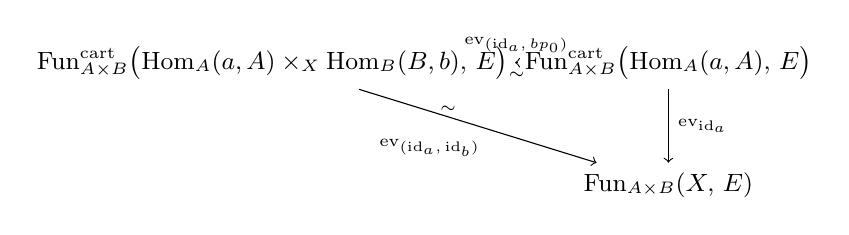
\begin{tikzpicture}[x=1.3em,y=1.3em,every node/.style={font=\small}]
  \node (TL) at (0,1.7) {$\mathrm{Fun}_{A\times B}^{\mathrm{cart}}\bigl(\mathrm{Hom}_{A}(a,A)\times_{X}\mathrm{Hom}_{B}(B,b),\,E\bigr)$};
  \node (TR) at (11.0,1.7) {$\mathrm{Fun}_{A\times B}^{\mathrm{cart}}\bigl(\mathrm{Hom}_{A}(a,A),\,E\bigr)$};
  \node (BR) at (11.0,-1.7) {$\mathrm{Fun}_{A\times B}(X,\,E)$};
  \draw[->] (TL) -- node[above]{$\scriptstyle\mathrm{ev}_{(\qcor{\mathrm{id}_{a}},\,\qcor{bp_{0}})}$} node[below]{$\scriptstyle\sim$} (TR);
  \draw[->] (TL) -- node[below left,pos=0.55]{$\scriptstyle\mathrm{ev}_{(\qcor{\mathrm{id}_{a}},\,\qcor{\mathrm{id}_{b}})}$} node[above left,pos=0.45]{$\scriptstyle\sim$} (BR);
  \draw[->] (TR) -- node[right]{$\scriptstyle\mathrm{ev}_{\qcor{\mathrm{id}_{a}}}$} (BR);
\end{tikzpicture}
\end{center}
\end{proof}

与\cref{cor:generalized-yoneda-lemma}一样，我们把\cref{thm:two-sided-yoneda-lemma}
解读为：它为双侧纤维化这一子范畴的包含定义了一个左双伴随，把跨度
$A\overset{a}{\leftarrow}X\overset{b}{\rightarrow}B$ 送到%
\cref{def:represented-two-sided-fibration}中所构造的那条\trTwoSidedIsofibration{}。当跨度
由单个非恒同\trFunctor{}表示时，人们也许会更青睐\cref{thm:two-sided-yoneda-lemma}
的一个「单侧」版本——它的确立要简单得多：

